%!TEX root = ../../msc17-game-book.tex

\phChapterWorksheet{Mummy Madness}{Main Puzzle 3}

Halloween is just no fun for Marvin. Everyone else gets to dress up in costumes, but Marvin is tired of wearing the same mummy outfit that he wears everyday. This year is going to be different though! Marvin has decided to enter Count Calcula's Annual Costume Contest and he is determined to win.

Since good *always* defeats evil, Marvin has decided that the best costume will be a superhero! Obviously in order to pull this off, Marvin needs a super belt.

``On my belt, I'm going to have five super symbols representing: strength, heart, persistence, benevolence, and the power to FLY (duh!). I want lines connecting each super symbol to each of the other super symbols, but I do NOT want those lines to cross! They can go around or behind on the back of the belt, but I don't want the lines crossing over each other anywhere! Can you help me??''

It looks like Marvin is tired of having all of his mummy wrapping crossing over itself..

``Amp'd squad! I'm giving you an inner tube and some markers to work with. If you can draw on that tube and show me how to make my belt work, I'm POSITIVE I can defeat Count Calcula in the costume contest! I am so positive that I'll even reward you with a puzzle piece if you help me!''

    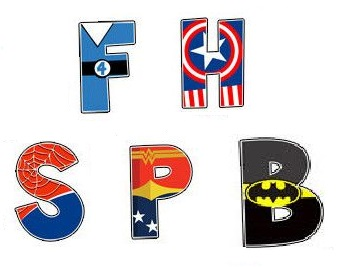
\includegraphics{assets/kat/alpha1}


Challenge Overview
\begin{itemize}
\item[*] Draw the 5 super symbols on the inner tube with a total of 10 lines connecting each symbol to all of the other symbols in such a way that no two lines cross over each other.

\item[*] When you think you've got it, go and present your solution to Marvin in \textbf{Challenge Room X}!
\end{itemize}
